\section{☞ Welcome to the Peeragogy
Workbook!}\label{welcome-to-the-peeragogy-workbook}

This booklet is designed to introduce you to our fun, exciting world of
peer learning and peer production!! You may already be familiar with
these terms, or they may be new to you. Either way, don't worry!!!

If they are new, consider the following 2 examples.

\begin{enumerate}
\def\labelenumi{\arabic{enumi}.}
\item
  \emph{Peer learning}: Joe Corneli needs to get from the suburbs of
  Chicago to the north side of the city. He gets on the commuter train
  and transfers to the purple ``L'' at Davis Street in Evanston. He
  plans to change to the red line at Howard Street, but the train says
  ``Loop'' and he asks another passenger whether it will stop at Howard.
  She says it will, but that he can save an hour of his time by riding
  express to the city and then coming back two stops! Joe makes it to
  his meeting with Charlie with plenty of time to spare.
\item
  \emph{Peer production}: Two cavewomen see lightning strike a tree and
  produce fire! Walking up to it they notice the heat and think
  ``Wouldn't it be nice to have fire for our family at night!'' Once the
  rain clears, they find some dry sticks and start working together to
  figure out how they can use them to start their own flame. After hours
  of trial and error, BOOM they've got fire! The news travels fast. :)
\end{enumerate}

Peeragogy is an approach to learning and working together on projects
ranging from the mundane to the monumental. Peer learning and peer
production are probably as old as humanity itself, but they take on new
importance in the digital age.

The Peeragogy Project is an informal learning project with members
worldwide. Three members of the project share their welcoming messages
below.

\textbf{Paola Ricaurte Quijano}: Welcome to the Peeragogy Project! We
are a group of enthusiastic people who love to learn and are trying to
find the best ways to learn together.

\textbf{Lisa Snow MacDonald}: Welcome to peeragogy! It's kind of a weird
name, but it's enormously powerful in providing a fresh understanding of
ways of working together.

\textbf{Dorotea Mar}: Your contributions will be really welcome if you
participate respectfully and harmoniously with other peers. It can
change your life and improve your well­being and make everything better.

\section{A Peeragogy Interview}\label{a-peeragogy-interview}

\subsection{Introductions}\label{introductions}

\textbf{Paola Ricaurte Quijano}: Hi! I'm Paola, I'm from Ecuador. I work
at Tecnológico de Monterrey, a private university in Mexico City, and I
love to learn with everybody!

\textbf{Dorotea Mar}: Hello. I'm in Berlin now and I really like the
peeragogical atmosphere of collaboration and I think we are really
improving ways of collaboration and peer production, so that's why I'm
here.

\textbf{Lisa Snow MacDonald}: Hello. This is Lisa from Los Angeles. My
background is media psychology and I'm interested in peeragogy as it
relates to business.

\emph{What is peer learning/production?}

\textbf{PRQ} Well, peer learning. learning with peers, learning from
peers and trying to make things together or make things happen together.
I think that for me, the most important thing I've learned from this
experience is that you can achieve more when you work together and set
goals together.

\textbf{LSM} I think what peeragogy does is it allows us to recognize
the value of those connections. A lot of other ways of working are more
individualized. It goes back to a concept of 1 + 1 = 2, which is very
rational and very measured and is kind of a dominant way of thinking in
our society today, whereas peer to peer learning and production
recognize the value of those connections. You may not be able to measure
it with a yardstick, but we understand that there is value in those
connections. So it's basically acknowledging that when it comes to
learning/collaborative environments if constructed the right way if
working well it can be 1 + 1 = 3 or 1 + 1 = 4. That type of situation,
which is really different from the way we're used to thinking about
things. And I think that's really the value of what we're doing and the
potential of what we could hopefully unlock.

\emph{More specifically, what is peeragogy and/or what is the Peeragogy
Project?}

\textbf{PRQ} This is a project that began spontaneously. We didn't have
a plan at the beginning. We just talked about the things that concerned
us the most. What do you need if you want to learn with others, how to
learn better? what do you want to learn? Where do you want to learn?
When do you want to learn? Basic questions that can be answered in many
ways. We don't have a strict line. We have a map, maybe, but a map that
can be walked through by many different paths. Paths that you choose can
be related to the people you are working with. I think it's been a great
experience for us. As Lisa said, we have been recognizing the talents
and strengths of every person that has contributed to and participated
in this project.

\textbf{LSM} OK. I'll take my best shot with this. Going back to what I
said earlier and building off what other people have said. Because we
don't have a good mental construct of how this works, and measurement is
difficult. We haven't learned how to measure these connections. I think
what peeragogy and the Peeragogy Project can do is it can establish what
people have said about focusing on the process. It can help people
understand the process better. Because this lack of structure can be
uncomfortable for people. We need to understand when that discomfort is
acceptable, so they don't revert and become counter­productive
participants in the process. The map analogy that Paola just mentioned,
is really good too. It's not about providing a direct path. If you're on
a trip trying to get from LA to Chicago, there's many paths you can
take. It's making sure you're monitoring your resources and you're
taking care of things along the way. You can drift off-course. One plus
one can equal zero if things don't work out well. So, what peeragogy and
the Peeragogy Project can do is to provide some structure and framework
around the unstructured way that things can be done. People trying to
make sure their methods are constructive and beneficial now have some
guidelines and things to watch out for.

\begin{center}\rule{0.5\linewidth}{\linethickness}\end{center}

\subsection{Example: Howard Rheingold Grows a Learning
Network}\label{example-howard-rheingold-grows-a-learning-network}

``When I started using social media in the classroom, I looked for and
began to learn from more experienced educators. First, I read and then
tried to comment usefully on their blog posts and tweets. When I began
to understand who knew what in the world of social media in education, I
narrowed my focus to the most knowledgeable and adventurous among them.
I paid attention to the people the savviest social media educators paid
attention to. I added and subtracted voices from my attention network,
listened and followed, then commented and opened conversations. When I
found something I thought would interest the friends and strangers I was
learning from, I passed along my own learning through my blogs and
Twitter stream. I asked questions, asked for help, and eventually
started providing answers and assistance to those who seemed to know
less than I. The teachers I had been learning from had a name for what I
was doing --- ``growing a personal learning network.'' So I started
looking for and learning from people who talked about HOW to grow a
``PLN'' as the enthusiasts called them.''

\begin{center}\rule{0.5\linewidth}{\linethickness}\end{center}

\emph{How do you do peeragogy?}

\textbf{DM} I think I do a lot of peeragogy and I'm very happy about it
because I learn so much from my group and from myself in this group that
I like to apply it to other projects that I'm in or things like
co­working and co­living projects. Especially the principle of mutual
respect that still remains after a very long time. And the way we relate
to each other is really nice.

The main principle is mutual respect and openness, and the process. And
in each detail, there is value that we believe in.

Let's say how we manage the Peeragogy Page or Community (See ``How to
Get Involved,'' later in this chapter.). These seem to be details, but
they're actually really important. So if we pay attention to all these,
every little thing matters, and this is how I do it. I try to be very
mindful in all interactions.

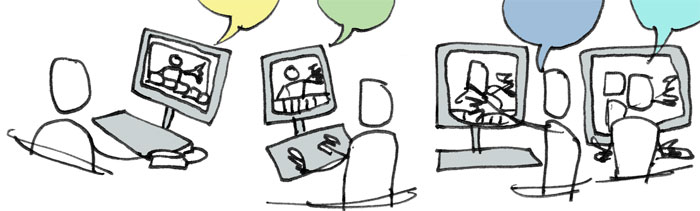
\includegraphics{../pictures/talking.jpg}

image

\begin{center}\rule{0.5\linewidth}{\linethickness}\end{center}

\subsection{Example: Learner, know
thyself.}\label{example-learner-know-thyself.}

When he joined the Peeragogy project in 2012, Charles Jeffrey Danoff did
a brief self­evaluation about what makes him interested in learning:

\begin{enumerate}
\def\labelenumi{\arabic{enumi}.}
\item
  Context. As a student, I resisted being groomed for some unforeseeable
  future. I'd rather work toward a specific goal.
\item
  Timing and sequence. I find learning fun when I'm studying something
  as a way to procrastinate another pressing assignment.
\item
  Social reinforcement. Getting tips from peers on how to navigate a
  snowboard around moguls was more fun for me than my Dad showing me the
  proper way to buff the car's leather seats on chore day.
\item
  Experiential awareness. In high school, it was not fun to sit and
  compose a 30-page reading journal on Frankenstein. But owing in part
  to those types of prior experiences, I now find writing pleasurable
  and it's fun to learn how to write better.
\end{enumerate}

\begin{center}\rule{0.5\linewidth}{\linethickness}\end{center}

\textbf{PRQ} I think peeragogy is more like a mind­set. I think we have
to change the way we interact with others and the way we understand the
parameters of learning. For example, I'm a teacher and, of course, my
teaching practice promotes collaborative, creative learning. So, I
expect my students to take responsibility for their own learning by
making decisions about most aspects of the learning process; to program
their own learning goals. They need to learn to effectively employ the
environments (like whiteboards), the activities, and the assessments.
I'm trying to give my learners the tools to decide how, what, and why
they want to learn. For me, it's been a very interesting experience.
Learners often find it unfamiliar to make their own decisions about the
process in a formal environment. At the beginning of the semester,
students are given everything and usually just follow guidelines and
criteria. I have been trying to change this dynamic. Students feel
insecure, because they really do not know how or what they want to do.
So, that process of making decisions together becomes very rich and very
meaningful.

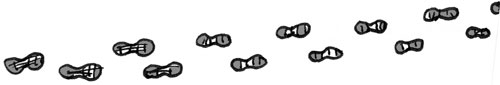
\includegraphics{../pictures/footprints.jpg}

image

\begin{center}\rule{0.5\linewidth}{\linethickness}\end{center}

\subsection{Example: Metacognition and
Mindfulness}\label{example-metacognition-and-mindfulness}

\begin{quote}
Alan Schoenfeld: ``What (exactly) are you doing? Can you describe it
precisely? Why are you doing it? How does it fit into the solution? How
does it help you? What will you do with the outcome when you obtain it?
'' {[}1{]}
\end{quote}

\begin{center}\rule{0.5\linewidth}{\linethickness}\end{center}

\emph{When do you do peeragogy?}

\textbf{DM} I think I'm always practicing it. I really like that during
the weekly hangouts we don't usually have rigid agendas. We just get
creative and let ideas connect and flow. And whatever happens it's the
right thing. We just work together and somehow the right things happen.
I think we're always doing peeragogy when we pursue activities and
projects in open, collaborative ways without imposing too much structure
or heirarchy.

\textbf{PRQ} I agree with Dorotea. The where and when questions are
related. If you're thinking about where, you're thinking about when. So
if ``where'' is everywhere, and ``when'' is always, I agree. Anywhere,
everywhere, all the time. It's an ongoing process. If you believe in
peeragogy as a way of doing things or making things happen, you cannot
switch back and forth betweeen two different personas and say, ``I'm not
working with peeragogy now,'' or ``I am applying peeragogy now.''

\textbf{LSM} I'm familiar with the business world where there are
distinct personalities. For example there are people who tend to be more
collaborative just by nature, who tend to adapt and to prefer a
peeragogical model. Other personalities are less so, and that's why what
we're doing here is valuable. In practice, there's seldom a conscious
recognition of these different styles of working. In a business
environment, there are different motivators, different personalities
tossed together, all united by a single goal. So understanding
peeragogical vs. heirarchical practices, and raising the differences to
the surface, could be very valuable in pursuing the goal of making
people's lives better in the business environment.

\textbf{DM} There are many collaborative projects that aim to do
something similar to this, but, in a sense, focus on different aspects
of the process, and maybe not on such an abstract level as we might.

Some people have natural peeragogical tendencies, and some people are
less transparent in the way they do things. For me, peeragogy is really
beneficial, especially for collaborative projects. Everybody works and
learns differently, so if everyone became increasingly aware of how they
and others work and learn, of how peergogy functions, and how it all
fits into a bigger picture, many tasks would not only be more
efficiently done, but also much more enjoyable. It's also beneficial if
everyone focusses on a bigger picture instead of focussing only on their
part of it, and if attention is drawn to all that could be done in a
peeragogical way.

\begin{center}\rule{0.5\linewidth}{\linethickness}\end{center}

\subsection{Example: Jay Cross on Setting
Sail}\label{example-jay-cross-on-setting-sail}

``If I were an instructional designer in a moribund training department,
I'd polish up my resume and head over to marketing. Co­learning can
differentiate services, increase product usage, strengthen customer
relationships, and reduce the cost of hand­holding. It's cheaper and
more useful than advertising. But instead of just making a copy of
today's boring educational practices, build something based on
interaction and camaraderie, perhaps with some healthy competition
thrown in. Again, the emphasis should always be on learning in order to
do something!''

\begin{center}\rule{0.5\linewidth}{\linethickness}\end{center}

\emph{Why do you do peeragogy?}

\textbf{PRQ} Why? Well, as said before, I believe in peeragogy. I
believe it's a good way to learn. Maybe it's the best way. I think I
wasn't aware of that before joining the group. I have always been a
self­learner, I have been working mostly alone. After I began working
with the group, I understood that you grow working with a group. You
achieve things that you aren't able to achieve alone. I think there's a
growing awareness of the value of collaboration in every setting and
environment. There are more and more learning communities around the
world where people are also learning that making decisions together and
working together are the best way to be in this world! I think as we
live through hard times, we increasingly need a sense that we are not
alone and that we cannot solve problems alone.

\emph{How did you join the Peeragogy project?}

\textbf{PRQ} After taking Howard Rheingold's course on Mind Amplifiers
in 2012 we were invited to join this group. There was no plan, just an
open question of how to best learn with others.\\
That's how it began. We had lots of sessions and discussed a wide range
of issues. The Peeragogy Handbook (http://peeragogy.org) was the product
of that process. We've been working with the Handbook, releasing a new
version every year and trying to figure out what might be the best way
to go forward and what the future of our collaboration as a group/team
might be.

\textbf{LSM} A couple friends of mine were involved in P2P learning.
They were invited to a conference at UCI. Howard was at the event and
they were familiar with him and his work. We ended up in an obscure
classroom and he started talking about principles that were peeragogy
related, while I don't know if it provided much value to my friends, it
sounded a lot like what I saw in business and he mentioned the group. So
after that, I met everyone here and it's been pretty random.

\textbf{DM} I think many paths led to my involvement. I have a lot of
academic experience and was doing research on Open Science. I had always
wanted to improve the way things work and somehow I wanted to do it more
creatively. I resonated a lot with the Peeragogy Project on many levels,
so somehow I just joined, I think it was serendipity of some kind.

This interview was conducted on December 15th, 2014. The transcript was
edited. You can watch the whole interview online at
http://is.gd/peeragogyworkbook\_interviews. (49 Minutes)

We've given you some examples but this wouldn't be a proper workbook
without an exercise. Pick at least one thing you're good at and one
thing you want to improve on from the selection below (or write in your
own alternative answers):

\begin{center}\rule{0.5\linewidth}{\linethickness}\end{center}

\section{Exercise: How do you see yourself fitting
in?}\label{exercise-how-do-you-see-yourself-fitting-in}

\subsection{Potential roles in your peer­learning
project}\label{potential-roles-in-your-peerlearning-project}

\begin{itemize}
\tightlist
\item
  Worker, Team Member, Co­Manager, Manager, Co­Leader, Leader
\item
  Reviewer, Editor, Author, Content Processor, Content Creator,
\item
  Presentation Creator, Designer, Graphics, Applications
\item
  Attendee, Participant, Coordinator, Project Manager, Planner
\item
  Mediator, Moderator, Facilitator, Proponent, Advocate, Representative,
  Contributor , Activist,
  {~~~~~~~~~~~~~~~~~~~~~~~~~~~~~~~~~~~~~~~~~~~~~~~~}
\end{itemize}

\subsection{Potential contributions}\label{potential-contributions}

\begin{itemize}
\tightlist
\item
  Create, Originate, Research, Aggregate
\item
  Develop, Design, Integrate, Refine, Convert
\item
  Write, Edit, Format,
  {~~~~~~~~~~~~~~~~~~~~~~~~~~~~~~~~~~~~~~~~~~~~~~~~}
\end{itemize}

\subsection{Potential motivations}\label{potential-motivations}

\begin{itemize}
\tightlist
\item
  Acquisition of training or support in a topic or field;
\item
  Building relationships with interesting people;
\item
  Finding professional opportunities through other participants;
\item
  Creating or bolstering a personal network;
\item
  More organized and rational thinking through dialog and debate;
\item
  Feedback about performance and understanding of the topic.
\item
  {~~~~~~~~~~~~~~~~~~~~~~~~~~~~~~~~~~~~~~~~~~~~~~~~~~~~~~~~~~~~~~~~~~~~~~~~~~~~~~~~~~~~~~~~~~~~~~~~~~~~~~~~~~~~~~~~~~~~~~~~~~~~~~~~}
\end{itemize}

\begin{center}\rule{0.5\linewidth}{\linethickness}\end{center}

Visuals by Amanda Lyons (http://visualsforchange.com/). Booklet by
Charlie Danoff, Paola Ricaurte Quijano, Lisa Snow MacDonald, Dorotea
Mar, Joe Corneli and Charlotte Pierce.

Prepared for Public Domain Day 2015 on January 1st, 2015.

See \url{https://github.com/Peeragogy/Peeragogy.github.io} for the
``behind the scenes''.

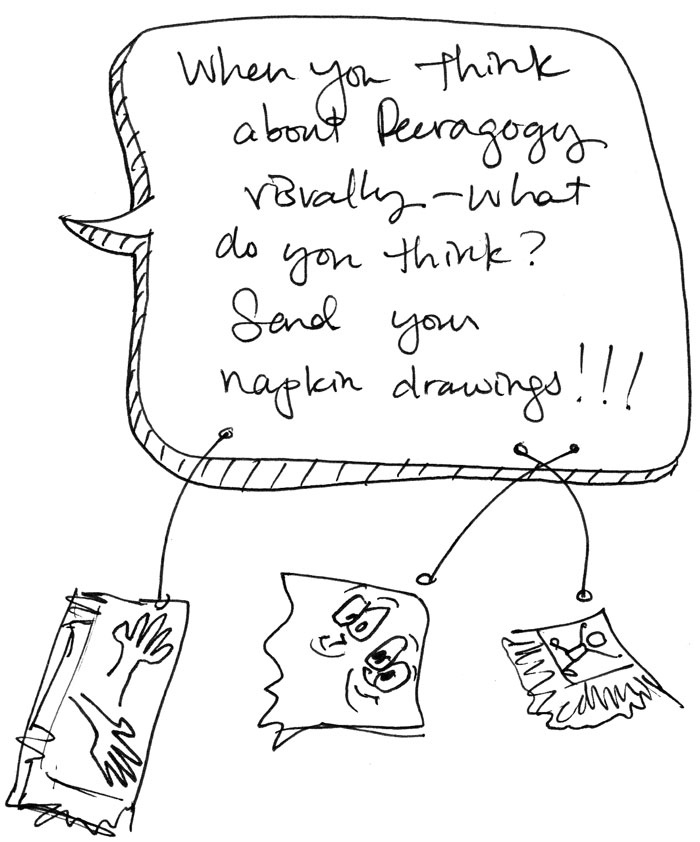
\includegraphics{../pictures/napkin-drawings.jpg}

image

\section{Reference}\label{reference}

\begin{enumerate}
\def\labelenumi{\arabic{enumi}.}
\tightlist
\item
  Schoenfeld, A. H. (1987). What's all the fuss about metacognition? In
  A. H. Schoenfeld (Ed.), Cognitive science and mathematics education
  (pp. 189­215). Hilldale, NJ: Lawrence Erlbaum Associates.
\end{enumerate}
